\section{Theory}
\subsection{Ideal Crystals}\label{subsec:crystal_lattice}
To understand the sapphire substrate and \ac{zno} thin film crystal structure 
as well as \ac{hrxrd}, a fundamental understanding of the structure of crystalline solids 
is essential.
The following pages therefore serve as a summary of the concepts from solid-state physics relevant 
to this work.

\subsubsection{Bravais Lattice, Unit Cell, and Basis}
The model of an ideal crystal is used as an idealization for many solids.
According to \citeauthoryear{Hunklinger}, an ideal crystal is a three-dimensional, infinitely 
extended arrangement composed of identical, periodically repeating building blocks.
These building blocks are referred to as the basis.
They can represent individual atoms as well as complex atomic structures.
If one reduces each building block to a single point, a simple-to-describe point lattice is formed.
This lattice is subject to various symmetries, allowing the lattice to be classified.

A simple classification can be made using rotation axes.
Here, one considers the rotation operators $R_{\hat{e}}(2\pi / n)$ for an arbitrary axis $\hat{e}$ by
an angle of $2 \pi /n$ that map the point lattice onto itself.
The parameter $n \in \mathbb{N}$ is called the fold and divides the point lattices into seven different
crystal systems, which are listed in \cref{tab:crystal_systems} \autocite{Hunklinger}.

\begin{table*}
    \centering
    \begin{tabular}{c c c c}
        \toprule
        Crystal System           & Lattice Constants & Angles                                       & Fold \\ \midrule
        Triclinic                & $a \neq b \neq c$ & $\alpha \neq\beta \neq\gamma$                & 1          \\
        Monoclinic               & $a \neq b \neq c$ & $\alpha=\gamma=\ang{90},\beta \neq \ang{90}$ & 2          \\
        Orthorhombic             & $a \neq b \neq c$ & $\alpha=\beta=\gamma=\ang{90}$               & 2 (two)    \\
        Tetragonal               & $a = b \neq c$    & $\alpha=\beta=\gamma=\ang{90}$               & 4          \\
        Hexagonal                & $a = b \neq c$    & $\alpha=\beta=\ang{90}, \gamma=\ang{120}$    & 6          \\
        Trigonal (Rhombohedral)  & $a=b=c$           & $\alpha=\beta=\gamma \neq \ang{90}$          & 3          \\
        Cubic                    & $a=b=c$           & $\alpha=\beta=\gamma=\ang{90}$               & 3 (four)   \\ \bottomrule
    \end{tabular}
    \caption{Classification of the different crystal systems. \imcite{Hunklinger}}
    \label{tab:crystal_systems}
\end{table*}

Another important symmetry is translational symmetry.
Considering the translation operators $T(\mathbf{O})$ that map the lattice onto itself, one recognizes
the relationship $\mathbf{O} = n_{1}\mathbf{a}_{1}+n_{2}\mathbf{a}_{2}+n_{3}\mathbf{a}_{3}$ due to the periodicity of the lattice, where
$\mathbf{a}_{i}\in\mathbb{R}^{3}, n_{i}\in\mathbb{Z}, i\in \{1,2,3\}$ \autocite{Hunklinger}.
The vectors $\mathbf{a}_{i}$
define a skew-angled coordinate system and are called primitive lattice vectors.
They span a so-called three-dimensional Bravais lattice.
The distances between two adjacent lattice points, i.e., the magnitudes
$\lvert \mathbf{a}_{i} \rvert$, are called lattice constants \autocite{Ashcroft}.
Depending on how the crystal system behaves under symmetry operations, different conditions arise for
the lattice constants and the angles between the lattice vectors.
With the definition of a basis and a Bravais lattice, any ideal crystal can be described.
A crystal structure is built by placing identical copies of the basis at every point of the Bravais lattice
\autocite{Ashcroft}.

According to \citeauthoryear{Ashcroft}, by cleverly choosing subsets of real space, the entire space can be
filled completely without overlap by arranging these subsets next to each other.
Such sets are called unit cells.
If the unit cell is chosen to contain only one lattice point, it is called a primitive
unit cell.
With a primitive unit cell, the space can be tiled without gaps or overlaps by translating the cell
along each Bravais lattice vector.
A simple construction yields a parallelepiped spanned by the three basis vectors.
The volume $V_\mathrm{UC}= \lvert \mathbf{a}_1 \cdot (\mathbf{a}_2 \times  \mathbf{a}_3) \rvert$ of this
parallelepiped gives the effective volume per Bravais lattice point \autocite{Ashcroft}.

A further subdivision of the crystal systems can be made using the three-dimensional Bravais lattices.
These can be generated by operations of the point group and categorize periodic structures
into 14 different Bravais lattices \autocite{Grundmann}.
The lattices relevant to this work are presented below.

\subsubsection{Selected Crystal Lattices}\label{subsubsec:selected_crystal_lattices}
\begin{figure*}
    \centering
    \begin{subfigure}[t]{0.3\textwidth}
        \centering
        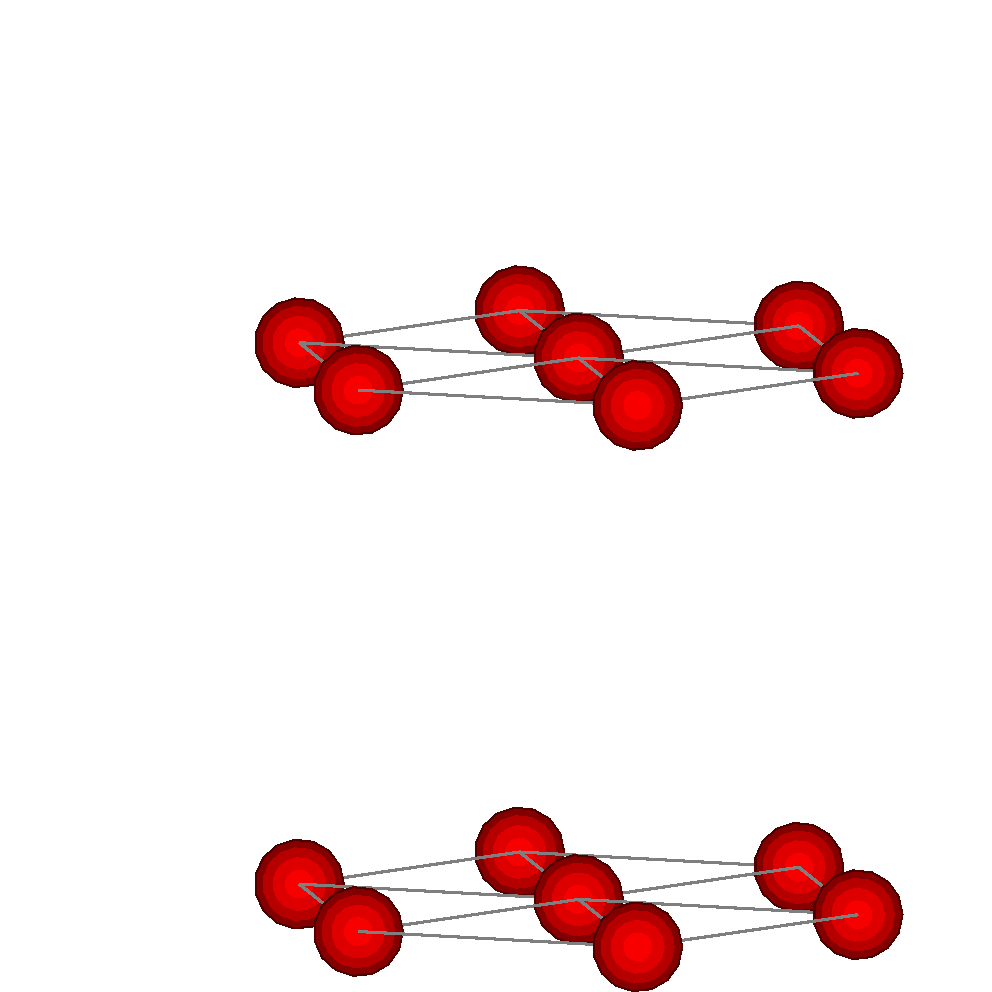
\includegraphics[width=\textwidth]{../assets/hex}
        \caption{hexagonal lattice} 
        \label{hex}
    \end{subfigure}
    \begin{subfigure}[t]{0.3\textwidth}
        \centering
        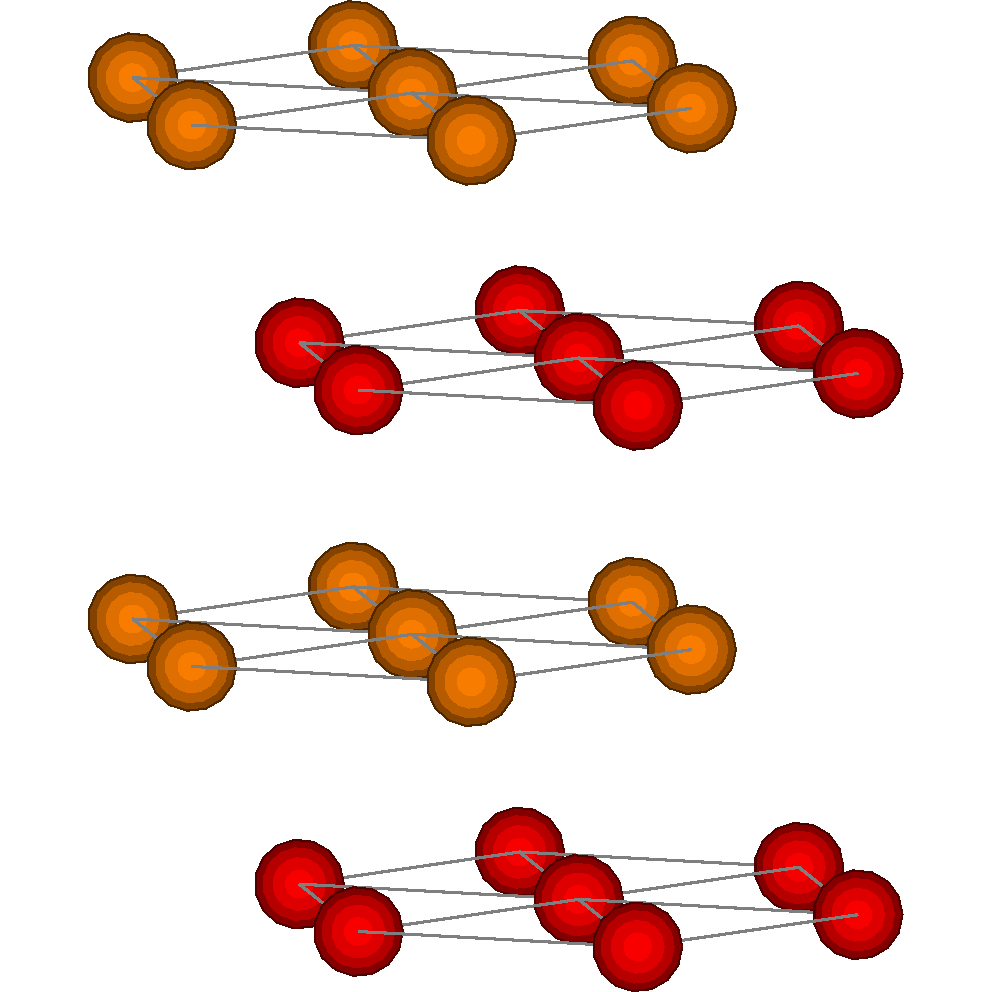
\includegraphics[width=\textwidth]{../assets/hcp}
        \caption{hcp lattice} 
        \label{hcp}
    \end{subfigure}
    \begin{subfigure}[t]{0.3\textwidth}
        \centering
        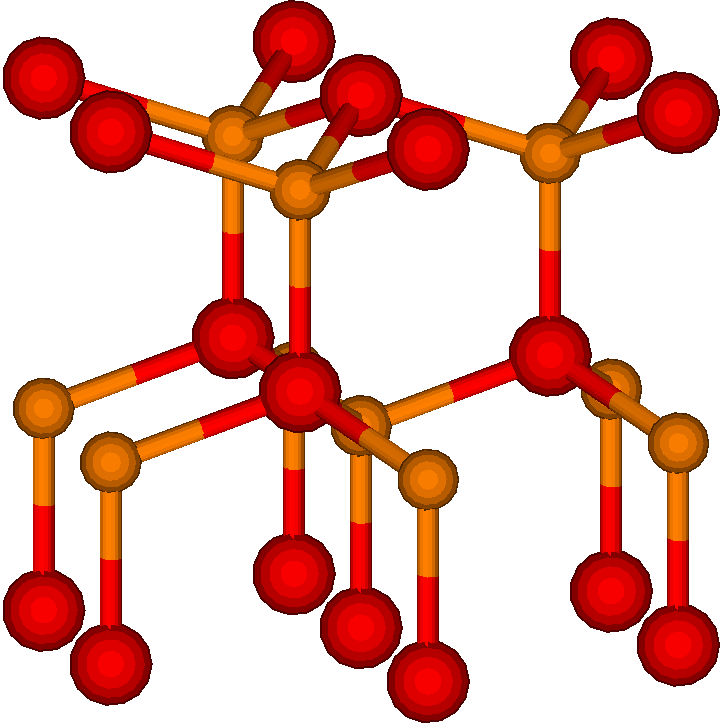
\includegraphics[width=\textwidth]{../assets/wurzite}
        \caption{Wurtzite lattice}
        \label{wurtzite}
    \end{subfigure}
    \caption{Selected crystal lattices for investigating \ac{zno}\label{fig:lattice_structures}}
\end{figure*}

\paragraph{Wurtzite Structure}
To understand the wurtzite structure, one first considers the simple hexagonal structure, defined by the primitive
vectors \autocite{Ashcroft}:
\begin{equation}
    \mathbf{a}_1 = a\hat{x}, \quad
    \mathbf{a}_2 = a/2 (\hat{x} + \sqrt{3} \hat{y}), \quad
    \mathbf{a}_3 = c \hat{z}.
    \label{eq:hex}
\end{equation}
This forms a lattice with points at the corners of a hexagon and at the centers of its hexagonal faces, as shown in \cref{hex}.
From the simple hexagonal structure, the hexagonal close-packed (hcp) structure arises.
This is based on a simple hexagonal lattice with a two-atom basis at the lattice positions $(0,0,0)$ and
$(\mathbf{a}_1/3 + \mathbf{a}_2/3 + \mathbf{a}_3/2)$, as shown in \cref{hcp} \autocite{Ashcroft}.
The wurtzite structure consists of a simple hexagonal lattice with a four-atom basis.
However, a better visualization is obtained by considering two stacked hcp lattices, shifted relative to each other by
a height of $\sqrt{3/8}a$ \autocite{Grundmann}, as depicted in \cref{wurtzite}.
\ac{zno} crystallizes in this structure.

\paragraph{Corundum Structure}
\begin{figure*}
    \centering
    \begin{subfigure}[t]{0.3\textwidth}
        \centering
        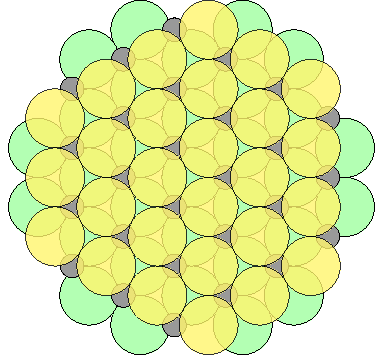
\includegraphics[width=\textwidth]{../assets/corundum_1.pdf}
        \caption{Two oxide layers with octahedral interstices between them. } 
        \label{hex}
    \end{subfigure}
    \begin{subfigure}[t]{0.3\textwidth}
        \centering
        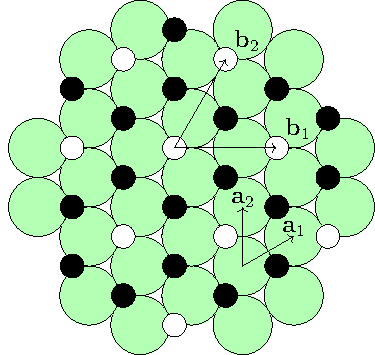
\includegraphics[width=\textwidth]{../assets/corundum_2.pdf}
        \caption{Bottom oxide layer and interstical mesh with aluminum submesh.} 
        \label{hcp}
    \end{subfigure}
    \begin{subfigure}[t]{0.3\textwidth}
        \centering
        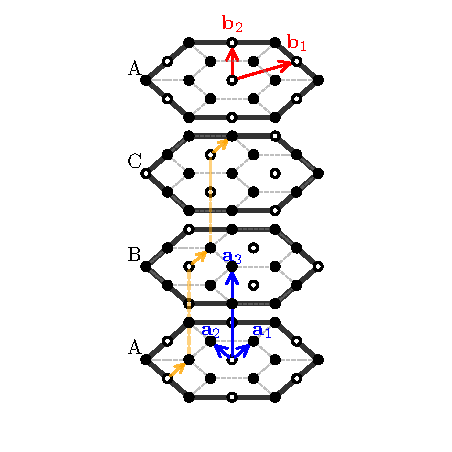
\includegraphics{../assets/corundum_3.pdf}
        \caption{3D view of interstical meshes with holes and aluminum atoms.}
        \label{wurtzite}
    \end{subfigure}
    \caption{Selected crystal lattices for investigating \ac{zno}\label{fig:lattice_structures}}
\end{figure*}
To describe the sapphire $\ce{Al2O3}$ structure, one starts with a hcp oxygen sublattice. 
In this structure, empty spaces between the closely packed oxygen atoms exist.
Since every empty space is surrounded by six oxygen atoms that form an octahedron, these spaces are 
referred to as octahedral interstices and depicted in \cref{fig:corundum}.
Most of these interstices are occupied by aluminum atoms.
The interstices lie on planes midway between two adjacent oxygen hcp layers.
Since the third hcp layer is directly above the first, the second interstical layer is directly above the first.
Therefore, all hexagonal interstical meshes are above each other, leading to a hexagonal arrangement 
of interstices. 

\Cref{fig:corundum_2} shows the arrangement of aluminum atoms in the in-plane interstical hexagonal 
mesh.
Since the number of interstices corresponds to the number of the oxygen layer below and since the 
stochiometry of aluminum oxide is $\ce{Al2O3}$, 2/3 of these interstices are occupied by aluminum atoms.
The remaining 1/3 of the interstices are empty and are called holes.
These holes are regions of negative localized charge. 
If one requires that the aluminum sublattice is ordered, there exist an in-plane solution since
one requires maximum separation between the holes due to their negative charge.
To fulfill this condition in-plane, the holes are arranged in a wider hexagonal "hole" mesh as a 
subset of the interstical mesh, as shown in \cref{fig:corundum_2}.

The arrangement of holes between adjacent meshes is not arbitrary. 
Again the requirement of an ordered sublattice with maximum separation between the holes uniquely 
determines the arrangement. 
The holes in adjacent meshes are shifted relative to each other in the direction of the closest packed
direction of the oxygen hcp lattice by a magnitude of an oxygen-oxygen distance. 
This out-of-plane shift of the holes is depicted in \cref{fig:corundum_3}.
Since a translation of 3 times the out-of-plane shift vector results in an identical arrangement, 
three different hole layers exist, that are labeled A, B, and C.
The oxygen meshes are labeled with '1' and '2' to distinguish between the two oxygen layers. 
The structural repeat unit of the corundum strucutre is then given by the sequence 1A2B1C2A1B2C, 
as shown in \cref{fig:corundum_4}, consisting of 6 oxygen layers. 


The reciprocal lattice plays a fundamental role in the further consideration of periodic structures.
The goal is to construct a function that is lattice-periodic in the Bravais lattice.
This function should therefore satisfy
$f(\mathbf{x})=f(\mathbf{x}+\mathbf{O})$, if $\mathbf{O}=\sum_{i=1}^{3} \alpha_{i}\mathbf{a}_{i}$.
Using a series expansion, the following general form is obtained:
\begin{align}
    f(\mathbf{x})&=\sum_{\mathbf{R}}a_{\mathbf{R}}\cdot \exp(\mathrm{i}\mathbf{R}\cdot\mathbf{x}), \notag\\
    f(\mathbf{x}+\mathbf{O})&=\sum_{\mathbf{R}}a_{\mathbf{R}}\cdot \exp(\mathrm{i}\mathbf{R}\cdot \mathbf{x})\cdot \notag
    \underbrace{ \exp(\mathrm{i}\mathbf{R}\cdot \mathbf{O}) }_{ \stackrel{!}{=}1 }  \\
    &\stackrel{!}{=} f(\mathbf{x}).
\end{align}
The necessary condition $\exp(\mathrm{i}\mathbf{R}\cdot \mathbf{O})=1$ is evident.
This is equivalent to the statement $\mathbf{R}\cdot \mathbf{O}=2\pi z$ with $z \in \mathbb{Z}$.
With this preliminary consideration, it is possible to define the reciprocal lattice by the set
$\{ \mathbf{R} \,\vert\, \exp(\mathrm{i}\mathbf{R}\cdot \mathbf{O})=1 \quad
\forall \mathbf{O} \in \text{span}(\mathbf{a}_{i}) \}$ \autocite{Ashcroft}.
Analogous to real space, primitive vectors can also be formed here with the following rule:
\begin{align}
    &\mathbf{b}_{1} = 2\pi \cdot \frac{\mathbf{a}_{2} \times \mathbf{a}_{3}}{V_{\mathrm{UC}}} \quad
    \mathbf{b}_{2} = 2\pi \cdot \frac{\mathbf{a}_{3} \times \mathbf{a}_{1}}{V_{\mathrm{UC}}} \\
    &\mathbf{b}_{3} = 2\pi \cdot \frac{\mathbf{a}_{1} \times \mathbf{a}_{2}}{V_{\mathrm{UC}}}.
\end{align}
Every point in the reciprocal lattice can be described by $\sum_{i=1}^{3} \beta_{i}\mathbf{b}_{i}$ with $\beta_i \in \mathbb{Z},
i\in\{1,2,3\}$.
The relation $\mathbf{b}_{i}\cdot \mathbf{a}_{j}=2 \pi \delta_{ij}$ holds,
where $\delta_{ij}$ is the Kronecker delta \autocite{Ashcroft}.

\subsubsection{Indexing of Lattice Planes and Directions}\label{subsubsec:indexing}
This section is based on the findings of \citeauthoryear{Ashcroft} \autocite{Ashcroft}.

The first important application of the reciprocal lattice is the characterization of lattice planes.
A lattice plane is any plane lying in the Bravais lattice that contains at least three non-collinear lattice points.
Due to crystal symmetry, infinitely many other lattice points lie within this plane.
Using translational symmetry, one can find parallel lattice planes separated by a distance $d$.
These are grouped together as families of lattice planes.

Families of lattice planes can be characterized using the reciprocal lattice, because for every
family of lattice planes with spacing $d$, there exist vectors of the reciprocal lattice that are perpendicular to the planes.
For a unique description, the shortest of these vectors, $\mathbf{r}$, is chosen, which always has the length $2 \pi / d$.
The converse is also true: for every vector $\mathbf{R}$ from the reciprocal lattice, there exists a family of perpendicular
lattice planes.
The spacing $d$ of these planes is linked to the magnitude of the smallest vector $\mathbf{r}$ parallel to $\mathbf{R}$ by
$\lvert \mathbf{r}\rvert=2\pi  /d$.
Thus, there is a simple way to uniquely identify lattice planes using reciprocal lattice vectors.

To label families of lattice planes, Miller indices are used.
Let $\mathbf{r}$ be the shortest reciprocal lattice vector perpendicular to the plane being characterized.
This can be represented as $ \mathbf{r} = h \mathbf{b_1} + k \mathbf{b_2} + l \mathbf{b_3}$.
The tuple $(h\, k\,l)$ are the Miller indices, which by definition must be integers.

There is a geometric interpretation that allows for the visualization of the indices in real space.
For every lattice plane, a corresponding $A$ can be found such that the plane equation $\mathbf{r} \cdot \mathbf{x} = A$
is satisfied.
Now, one defines the intercepts of the plane with the coordinate axes spanned by the primitive vectors $\mathbf{a}_i$ by the terms $x_{1}\mathbf{a}_{1}, x_{2}\mathbf{a}_{2}, x_{3}\mathbf{a}_{3}$.
Since the intercepts lie on the plane, the plane equation $\mathbf{r}\cdot(x_{i}\mathbf{a}_{i})=A$ is satisfied, and
with $\mathbf{r}\cdot\mathbf{a}_{1}=2\pi h$, $\mathbf{r}\cdot \mathbf{a}_{2}=2\pi k$,
$ \mathbf{r}\cdot \mathbf{a}_{3}=2\pi l$, the following relationship is found:
\begin{equation}
    x_{1}=\frac{A}{2\pi h}, \quad x_{2}=\frac{A}{2\pi k}, \quad x_{3} =\frac{A}{2\pi l}.
\end{equation}
If the axial intercepts $x_i$ are known, the Miller indices can be found by choosing the smallest possible parameter $A$
such that $h$, $k$, and $l$ are integers.

Not only lattice planes but also lattice directions can be indexed in a similar way.
The tuple $[h\,k\,l]$ describes the direction given by the vector $\mathbf{O} = h\mathbf{a}_{1}+k\mathbf{a}_{2}+
l\mathbf{a}_{3}$.
It should be noted that direction vectors in this context exist in real space,
whereas plane normal vectors are represented by vectors in reciprocal space.
To emphasize this, square brackets are used instead of round ones.
Furthermore, a special notation exists to denote equivalent families of lattice planes and directions.
In this context, this means that it is possible to transform equivalent families of planes and directions into one another through
symmetry operations.
Equivalent planes are denoted by $\{h \,k\, l \}$, and for directions, $\langle h\, k \, l \rangle$ is used accordingly.

\subsection{Crystal Defects}
    \begin{figure*}
        \centering
        \begin{subfigure}{0.3\linewidth}
            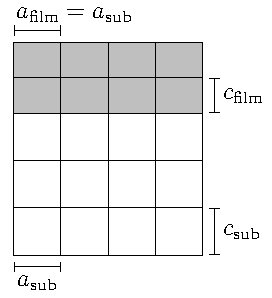
\includegraphics{../assets/pseudomorphic.pdf}
            \caption{Pseudomorphical growth of a thin film on a substrate}
        \end{subfigure}
        \begin{subfigure}{0.3\linewidth}
            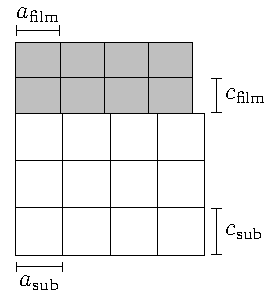
\includegraphics{../assets/partially_relaxed.pdf}
            \caption{Partially relaxed thin film on a substrate}
        \end{subfigure}
            \begin{subfigure}{0.3\linewidth}
            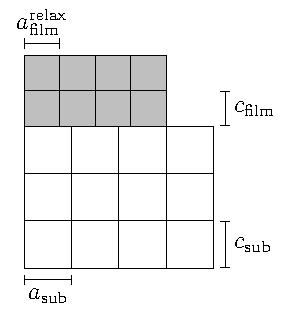
\includegraphics{../assets/fully_relaxed.pdf}
            \caption{Fully relaxed thin film on a substrate}
        \end{subfigure}
        \caption{(a) The unit cells of the substrate and the thin film are shown. The lattice constant 
        of the thin film is larger than that of the substrate. (b) The thin film is grown 
        pseudomorphically on the substrate. The in-plane lattice constant of the thin film is compressed 
        to match that of the substrate, while the out-of-plane lattice constant is expanded.}
    \end{figure*}